\section{Bayesian inference for MJPs}
%In practical situations, an MJP is noisily observed at
%a finite set of times. %with the observations themselves noisy. 
%This raises two questions: 
%%\begin{itemize}
%1) what is the underlying trajectory? and 2%)
%  what are the MJP parameters?
%%\end{itemize}
%  \vspace{-.1in}
\subsection{Trajectory inference given MJP parameters}
This was addressed in~\cite{RaoTeh13}, and extended to a broader class of 
jump processes %(like semi-Markov processes) 
in~\cite{RaoTeh12}. %Both center on alternate approaches to 
% Gillespie's algorithm, 
Both introduce auxiliary 
{\em candidate} jump times that are later {\em thinned}.  We focus on 
the simpler, more popular {\algname} algorithm~\cite{RaoTeh13},
based on the idea of {\em uniformization}~\cite{Jen1953}. 
%We refer to this as the Rao-Teh algorithm. % and describe it next.
%while in~\cite{RaoTeh12}, this was extended to a more general dependent thinning approach. 
%We outline
%the latter below: it is more general, and we are not aware of any work
%before~\cite{RaoTeh12} that describes it.

%Recall $A_i$ gives the 
%rate at which the MJP leaves $i$ for any other state. The
%parameters are set up so that self-transitions cannot occur. 
Uniformization simulates an MJP by introducing a parameter 
$\Omega \ge \max_i A_i$; \cite{RaoTeh13} suggest $\Omega = 2 \max_i A_i$. 
%Assuming the system is
%in state $i$, we sample a {\em candidate} transition-time from an
%exponential, now with rate $\Omega_i$. The system remains in state $i$
%until this time, after which it moves to state $j \neq i$ with probability
%$B_{ij} = A_{ij}/\Omega_i$. The system continues to remain in its current 
%state with probability $1-A_i/\Omega_i$. 
Unlike the sequential wait-and-jump Gillespie algorithm, first simulate 
a set $W$ of candidate
transition-times over $[0,t_{end}]$ from a rate-$\Omega$ 
Poisson process. $W$ %; these along with $0$ 
defines a random grid on $[0,t_{end}]$.
Define $B = \left(I +\frac{1}{\Omega}A\right)$; observe that this is a
stochastic matrix with positive elements, and rows adding up to $1$.
Assign state-values to the elements in $0 \cup W$ according to a discrete-time 
Markov chain with initial distribution $\pi_0$, and transition matrix $B$.
Call these states $V$. Thus $v_0 \sim \pi_0$, while $P(v_{k+1}=j|v_k=i) = B_{ij}$
for $k \in \{0,\cdots,|W|-1\}$.
Note that $\Omega > \max_i A_i$ results in more
candidate-times than actual MJP transitions; at the same time, unlike $A$, 
the matrix $B$ allows self-transitions. These two effects cancel
each other, and trajectories sampled this way for any $\Omega \ge \max_i A_i$
%These self-transitions correct for the extra candidate transition times
%produced by the higher rate $\Omega_i$, and~\cite{RaoTeh12} show that
%trajectories sampled this way 
have the same distribution as trajectories
sampled by Gillespie's algorithm~\cite{Jen1953,RaoTeh13}.
Introducing the thinned variables allowed~\cite{RaoTeh13} to develop
a novel and efficient MCMC sampler. At a 
high-level, each MCMC iteration 
samples a new grid $W$ conditioned on the trajectory $S(t)$, 
and then a new trajectory conditioned on the $W$. 
    ~\cite{RaoTeh13} show that the resulting Markov chain targets
    the desired posterior distribution over trajectories, and is 
    ergodic for any choice of $\Omega$ strictly greater than all the
    $A_i$'s. As mentioned earlier, \cite{RaoTeh13} suggest setting $\Omega = 2\max_i A_i$.
%The latter
%can be carried out using standard techniques from the discrete-time
%HMM literature.
\begin{algorithm}[H]
  \caption{The {\algname}~\cite{RaoTeh13} auxiliary variable Gibbs sampler for MJP trajectories}
   \label{alg:Unif_gibbs}
  \begin{tabular}{l l}
   \textbf{Input:  } & \text{MJP parameters $\theta$ and $\pi_0$, observations $X$}, 
                       \text{the previous path $S(t) = (S, T)$}.\\ 
                     & \text{A  parameter $\Omega > \max_i A_i$}, where
   $A = A(\theta)$ is the MJP rate-matrix.\\
   \textbf{Output:  }& \text{A new MJP trajectory $S' (t) = (S', T')$}.\\
   \hline
   \end{tabular}
   \begin{algorithmic}[1]
\State \textbf{Given the MJP trajectory $(S,T)$, sample a new set of thinned 
candidate times $U$}: %\cite{RaoTeh12} show that 
These are distributed as an inhomogeneous Poisson process with intensity 
$\Omega-A_{S(t)}$. Since the intensity is piecewise-constant, simulating it 
is straightforward.
\State \textbf{Given the thinned and actual transition times $W = (T \cup U)$
from the previous iteration (after discarding state information $S$), 
sample a new trajectory}:
    Conditioned on the skeleton $W$, the set of candidate jump
    times is fixed, and trajectory inference reduces to inference for
    a discrete-time hidden Markov model (HMM) with initial distribution
    $\pi_0$, and transition matrix $B$. \cite{RaoTeh13} use the forward-filtering
    backward-sampling (FFBS) algorithm, an efficient dynamic 
    programming algorithm that makes a forward pass through the
    finite set of times $W$, sequentially updating the 
    distribution over states at each time $w \in W$. 
    %at each time accounting for all observations in the previous interval. 
    Between any two consecutive elements of $W$,
    %separated by an interval $\Delta w$, 
    the system remain in a fixed state, with the likelihood for a state $i$ equal
    to the likelihood under state $i$ of all observations 
    in that interval. 
    %and a term $\Omega_i\exp(-\Omega_i\Delta t)$,
    %the probability that the next candidate time occurs after a wait
    %$\Delta t$ under state $i$.
    The end of the forward pass gives a distribution over states at the
    end time that accounts for all observations.
    The algorithm then makes a backward pass through the times in $W$, 
    sequentially sampling the state at each time given the state at the 
    following time, and the distribution over states calculated during the
    forward pass. 
\end{algorithmic}
\end{algorithm}

\subsection{Parameter inference for MJPs}
In practice, the MJP parameters themselves are unknown: often,
these are the quantities of primary interest when studying a dynamical
system. A Bayesian approach
places a prior $p(\theta)$ over these, and the
resulting posterior distribution $P(\theta|X)$ is approximated
with samples drawn by Gibbs sampling. In particular, for an arbitrary 
initialization of the parameters and the trajectory, one repeats the
two steps from algorithm~\ref{alg:MJP_gibbs}:
\begin{algorithm}[H]
  \caption{Gibbs sampling for parameter inference for MJPs}
   \label{alg:MJP_gibbs}
  \begin{tabular}{l l}
   \textbf{Input:  } & \text{A set of partial and noisy observations $X$}, \\
                      & \text{The previous MJP path $S(t) = (S, T)$, the previous MJP parameters $\theta$}.\\ 
   \textbf{Output:  }& \text{A new MJP trajectory $S' (t) = (S', T')$, 
                            new MJP parameters $\theta'$}.\\
   \hline
   \end{tabular}
   \begin{algorithmic}[1]
  \State  Sample a trajectory from the conditional 
  $P(S'(t)|X,S(t),\theta)$ by 
  algorithm~\ref{alg:Unif_gibbs}.
  \State Sample a new $\theta$ from the conditional 
    $P(\theta'|X,S'(t))$.
   \end{algorithmic}
\end{algorithm} 
\vspace{-.1in}
The distribution $P(\theta'|X,S(t))$ depends on a set of sufficient statistics of the 
MJP trajectory: how
much time is spent in each state, and the number of transitions
between each pair of states. 
%Given these, sample a new $\theta$ from the conditional $p(\theta|X,S(t))$. 
In special circumstances, $\theta$ can be directly sampled from its 
conditional distribution, otherwise, one has to use a Markov kernel like
Metropolis-Hastings or Hamiltonian Monte Carlo to update $\theta$ to 
$\theta'$. In any event, this introduces no new technical challenges.
%from the
%conditional $p(\theta_{new}|X,S(t),\theta_{curr})$. 
  \begin{figure}%[b]
  \centering
  \begin{minipage}[hp]{0.44\linewidth}
  \centering
    \vspace{-0 in}
    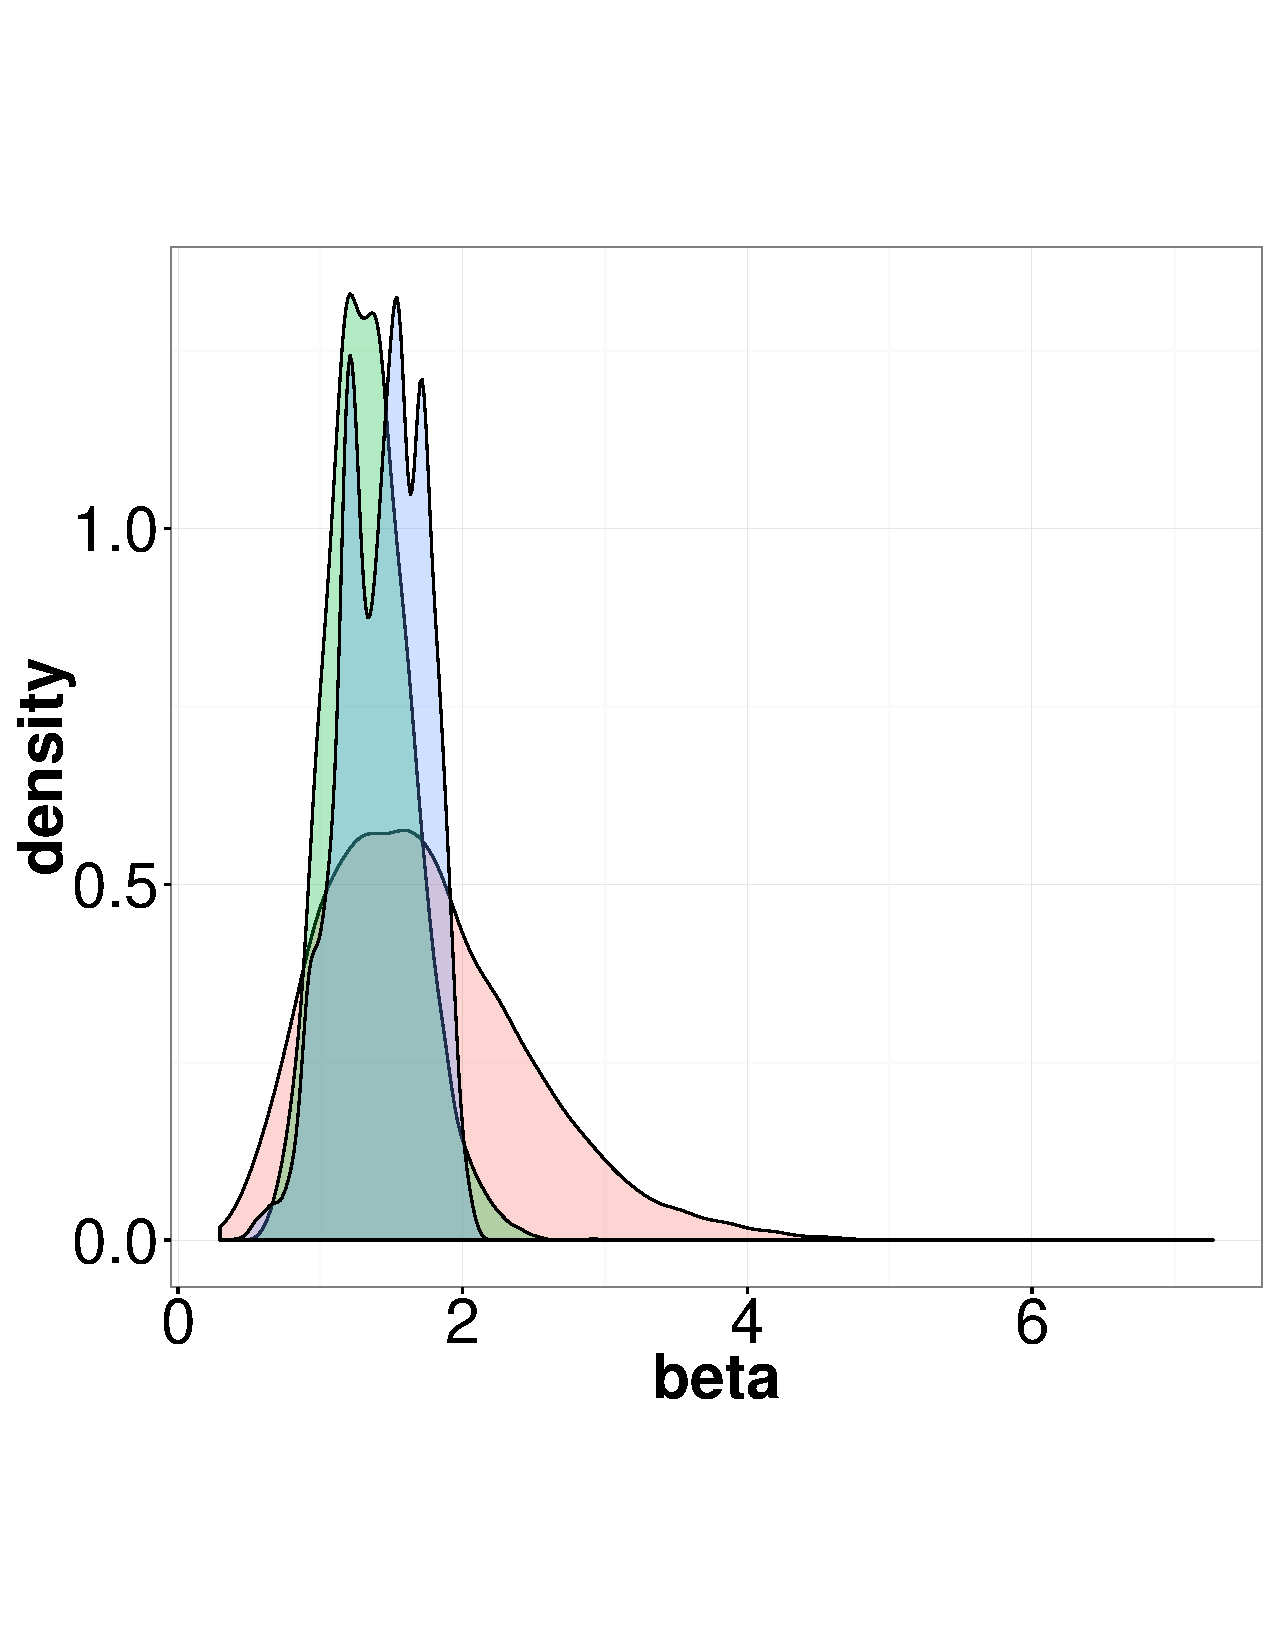
\includegraphics [width=0.7\textwidth, angle=0]{figs/dist_beta.pdf}
    \vspace{0.1 in}
  \end{minipage}
% \begin{minipage}[!hp]{0.4\linewidth}
% \centering
%   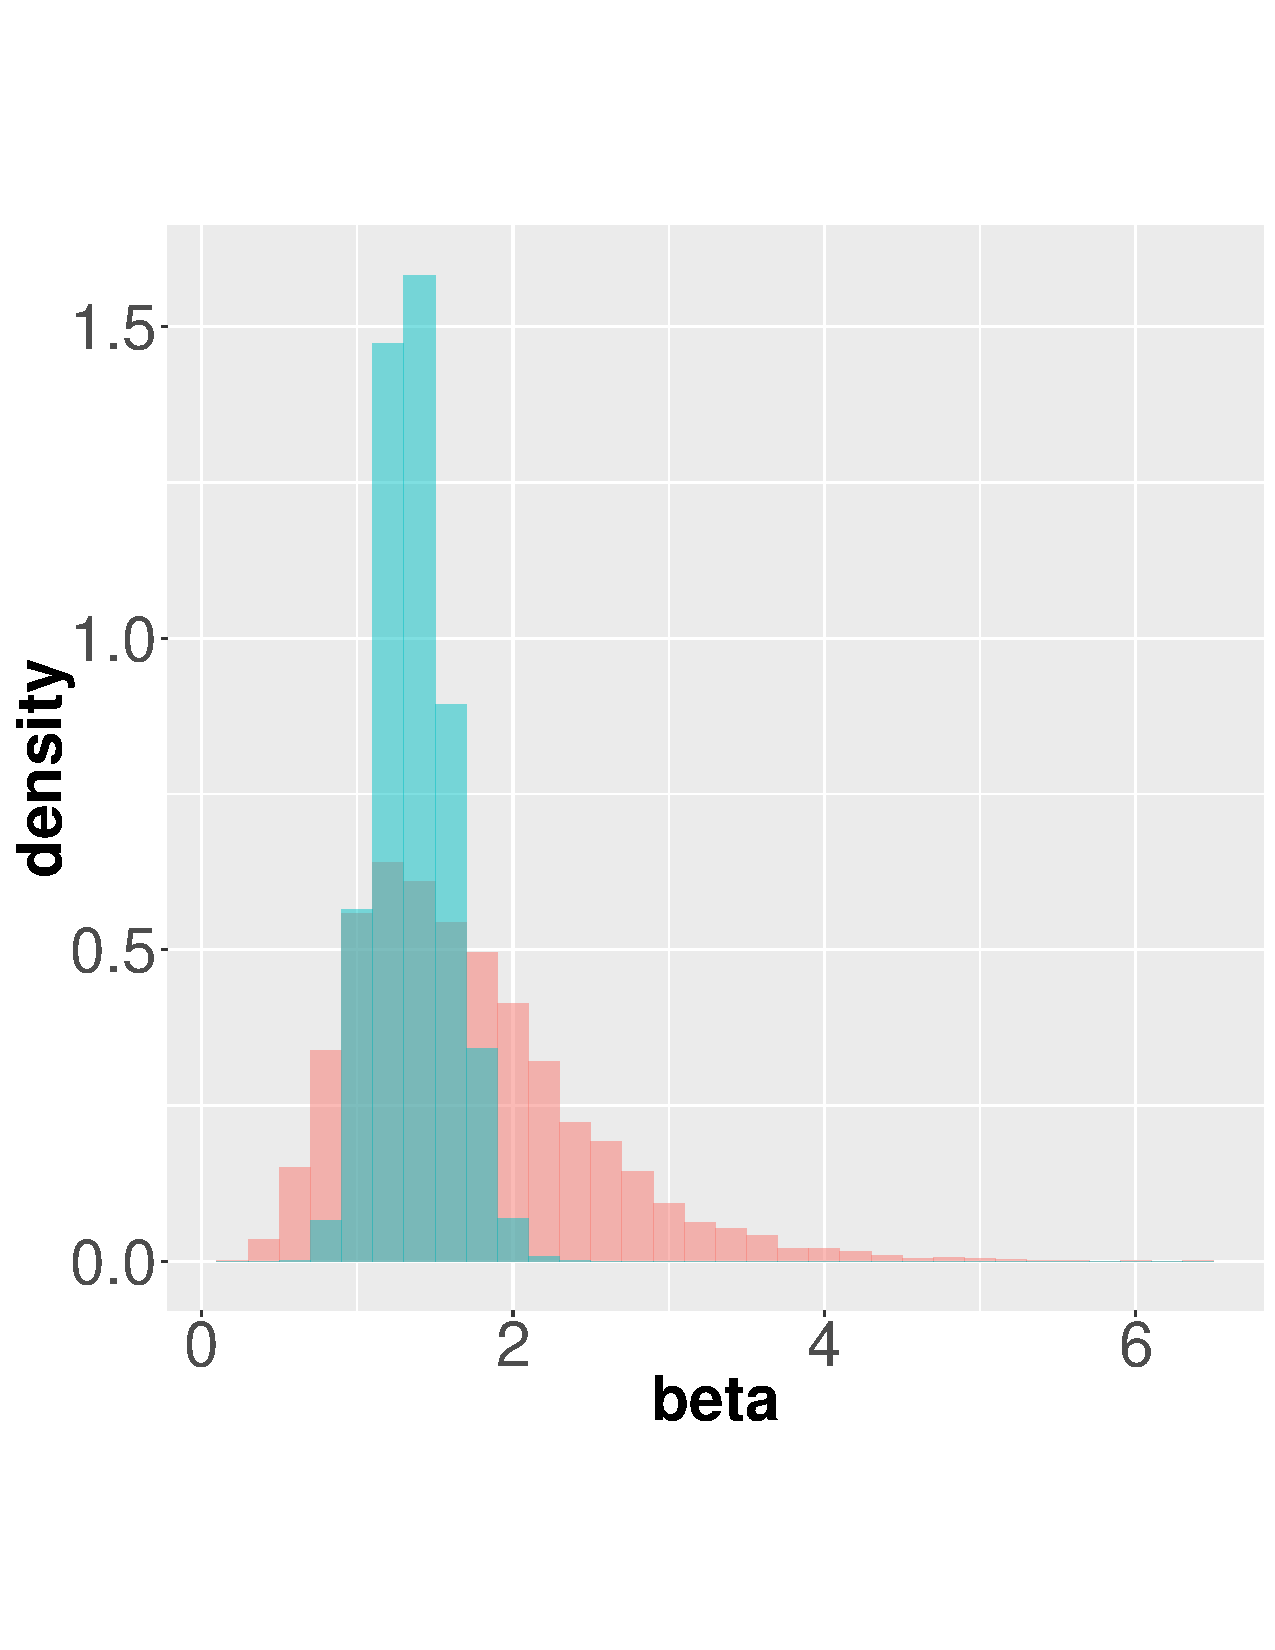
\includegraphics [width=0.90\textwidth, angle=0]{figs/hist_beta.pdf}
%   \vspace{-0 in}
% \end{minipage}
  \begin{minipage}[hp]{0.55\linewidth}
    \vspace{-0.3 in}
  \caption{Prior distribution of an MJP parameter (the wide red density),
  as well as two conditional distributions. Narrow dotted-green is the
density conditioned on both the observations as well as a simulated
MJP posterior. The wider dashed-blue curve is density of interest: the
marginal distribution of the paramters conditioned on observations. These
plots were produced from the experiment in section~\ref{sec:immig}.}
     \label{fig:hist}
  \end{minipage}
    \vspace{-0.6 in}
  \end{figure}
  However, the Gibbs sampling approach %of algorithm~\ref{alg:MJP_gibbs} 
  comes with a well-known limitation:
coupling between path and parameters can result in a very sluggish
exploration of parameter and path space. We illustrate this in figure~\ref{fig:hist},
which shows the posterior distribution of an MJP parameter (in dashed-blue)
%(this is the distribution of interest, conditioned only on the observations) 
is less concentrated than the distribution conditioned on both observations 
as well the MJP trajectory (dotted-green). 
%We have also included the prior distribution in red. 
%Observe that the latter is more concentrated than the former. 
The coupling is strengthened as the trajectory grows longer, and
the Gibbs sampler can mix very poorly for situations with
long observation periods, even if the observations themselves are
sparse and only mildly informative about the parameters.

For the discrete-time case, this problem of parameter-trajectory
coupling can be circumvented by marginalizing out the MJP trajectory 
and directly sampling from the posterior over parameters $P(\theta|X)$.
In its simplest form, this approach involves a Metropolis-Hastings
scheme that proposes a new parameter $\vartheta$ from some proposal 
distribution 
$q(\vartheta|\theta)$, accepting or rejecting according to the usual
Metropolis-Hastings probability. The latter step requires calculating the 
marginal probabilities $P(X|\theta)$ and $P(X|\theta')$, integrating out
the exponential number of possible latent trajectories. Fortunately
this marginal probability is a by-product of the forward-backward
algorithm used to sample a new trajectory, so that no 
additional computational burden is involved. 
%The overall algorithm then is:
\begin{algorithm}[H]
  \caption{Metropolis-Hastings parameter inference for a discrete-time 
Markov chain}
   \label{alg:disc_time_mh}
  \begin{tabular}{l l}
   \textbf{Input:  } & \text{Observations $X$};
   proposal density $q(\vartheta|\ctheta)$; 
   \text{previous parameters $\ctheta$ }.\\
   \textbf{Output:  }& \text{A new Markov chain parameter $\ntheta$}.\\
   \hline
   \end{tabular}
   \begin{algorithmic}[1]
  \State Propose a new parameter $\vartheta$ from the proposal distribution
  $q(\vartheta|\ctheta)$.
  \State Run the forward pass of the forward-backward algorithm to 
    obtain the marginal likelihood of the observations, $P(X|\vartheta)$.
    \State Set $\ntheta = \vartheta$ with probability 
    $\min(1,\frac{P(X,\vartheta)q(\ctheta|\vartheta)}{P(X,\ctheta)q(\vartheta|\ctheta)})$, else 
    $\ntheta = \ctheta$.
  \State Sample a new path with
    the backward pass of the forward-backward algorithm.
    %for the chosen parameter.
\end{algorithmic}
\end{algorithm}

\vspace{-.35in}
\subsection{A marginal sampler for MJP parameters} 
Constructing a marginal sampler over the MJP parameters by
integrating out the continuous-time trajectory is harder.
%the set of transition times is unbounded, with individual elements
%unconstrained over the observation interval $[0,\cT]$.
%Naively calculating this marginal probability for the continuous-time
%case is not straightforward, as there is no finite set of candidate
%times to make a pass over. 
One approach~\cite{FearnSher2006} makes a sequential 
forward pass through all {\em observations} $X$, using matrix exponentiation
to marginalize out all
continuous-time paths between successive times. As
shown in~\cite{RaoTeh13}, this approach is cubic rather than 
quadratic in the 
number of states, cannot exploit structure like sparsity in the 
transition matrix, and can depend in not trivial ways on the exact 
nature of the observation process.
Also, the number of expensive matrix exponentiations scales
with the number of observations rather than the number of transitions.
%
%
A second approach, particle MCMC~\cite{Andrieu10}, uses 
particle filtering to get an unbiased estimate of the marginal 
$P(X|\theta)$. Plugging this into the Metropolis-Hastings 
acceptance probability results in an MCMC sampler that targets the 
correct posterior, however %~\cite{Andrieu09}, 
the resulting scheme does not exploit the structure 
of the MJP, and we show that it is quite inefficient.

\cite{RaoTeh13, RaoTeh12} demonstrated the advantage of
introducing the thinned events $U$: this allows exploiting discrete-time 
algorithms like FFBS for efficient inference.
%be brought to playthe thinning-based approach over matrix exponential and particle-MCMC
%approaches for trajectory inference. 
In the next section, we outline a \naive\  first attempt at extending this 
approach to parameter inference.
We describe why this approach is not adequate, and then describe our
final algorithm. % in the section after. 
